\chapter{Quantum repeaters}
\label{sec:12_quantum_repeaters}
\label{ch:repeaters}

\section{The need for repeaters}
\label{sec:12-1_need_for_repeaters}

In the previous Chapter, we have seen that there is one big problem when trying to communicate over long distances, and that's photon loss in fibers.
The further that we are trying to communicate, the more likely we are to lose the photon.
There's also another problem, and that's the number of devices that are connected to the network. Currently (2022) there are 8 billion people, and an estimated 31 billion Internet of Things devices.
Despite this staggering number, all of these devices can communicate with each other.
How is this achieved?
One way is to establish a direct connection between each device that is present in the network as shown in the left panel of Fig.~\ref{fig:12-1_all_to_all}.
Two devices are connected by a single link.
Three devices require three links, four devices require six links and so on.
For $N$ devices, $N (N - 1) / 2$ links are needed in order to have all-to-all coupling.

\begin{figure}[t]
    \centering
    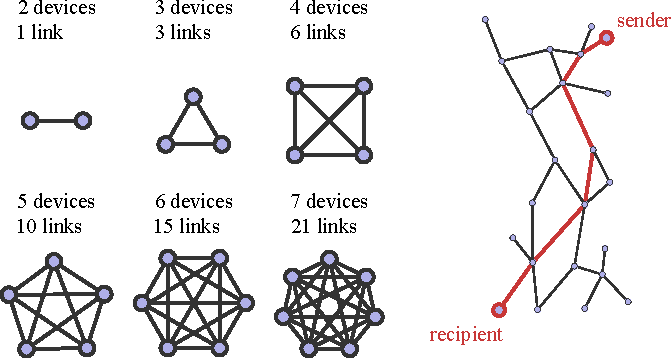
\includegraphics[width=0.85\textwidth]{lesson12/12-1_all_to_all.pdf}
    \caption[All-to-all coupling]{Right panel shows how many links are required to have all-to-all coupling. Left panel shows a more realistic network topology and the path along which a qubit needs to be teleported from sender to a receiver.}
    \label{fig:12-1_all_to_all}
\end{figure}

Real networks do not use all-to-all coupling.
Each individual link requires dedicated hardware that is allowing communication between two devices in the network.
Adding a single device to the network would also require to add links to all existing devices.
Such an approach is clearly not practical even for relatively small networks.
The right panel of Fig.~\ref{fig:12-1_all_to_all} shows a much more realistic network, where an arbitrary sender can still transmit a message to the intended receiver, even in the absence of a direct link between the two.

In quantum networks, information encoded in qubits is not transmitted directly.
Rather we use entangled pairs to teleport the state of the qubit as discussed in Chapter~\ref{sec:8_teleportation}.
Each link connecting two devices shares a Bell pair which is used to pass the state of the qubit carrying the quantum message from one device to the next.
We can go back to the right panel of Fig.~\ref{fig:12-1_all_to_all} and this time think of as a quantum network, where the quantum sender wishes to pass the state of a qubit to the recipient.
The state of the sender's qubit can be teleported hop-by-hop along the red path until it reaches the recipient.
A problem with this approach is that the operations required by the teleportation protocol as well as the memories used to store Bell pairs are not perfect.
This in turn decreases the fidelity of the teleported qubit.
Repeating the teleportation in this hop-by-hop approach deteriorates the fidelity further resulting in a completely garbled quantum state being teleported to the recipient.
A way around this problem is to use the link-level Bell pairs to create a direct entangled connection between the sender and the recipient so that the quantum state can be teleported in one hop.
The quantum nodes that achieving this splicing of link-level entanglement are called \textit{\textbf{quantum repeaters}}, and they are indispensable in the design of long-distance quantum networks.

We will address four requirements in this lesson.
First, we will show how to establish entanglement between neighboring nodes of a quantum network. This is known link-level entanglement.
Next, we will discuss how the link-level entanglement can be used to create a long-distance entangled connection between end nodes using entanglement swapping.
After this, we will deal with the issues presented by the adverse effects of noise.
Finally, we will look at management of networks, routing, multiplexing and resource management.


\section{Making link-level entanglement}
\label{sec:12-2_making_link_level_rantanglement}

In this section, we consider the task of creating link-level entanglement between two neighboring repeaters of a quantum network.
One way of entangling two quantum memories and creating link-level entanglement is pictured in Fig.~\ref{fig:12-2_MIM}, and is known as \textit{\textbf{memory-interfere-memory}} (MIM) link architecture.
Other names for this architecture are memory-interfere-memory or meet-in-the-middle.
Each repeater node is equipped with a quantum memory, and is coupled to an optical fiber.
The fibers lead to a \textit{\textbf{Bell state analyzer}} (BSA), an optical device which is capable of measuring incoming photons in the Bell basis.
We will discuss an implementation of the BSA in Section~\ref{sec:13-3_Bell_state_measurement_2}.

\begin{figure}[t]
    \centering
    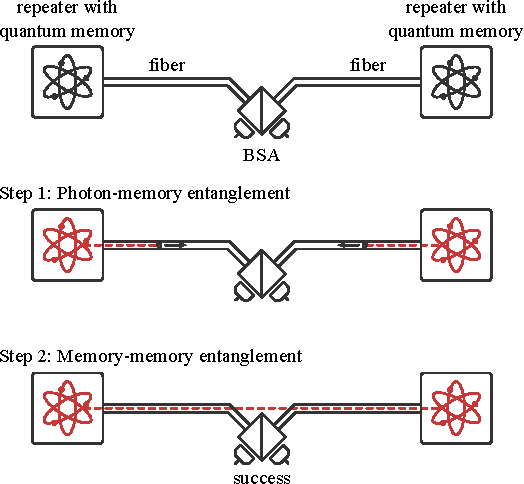
\includegraphics[width=0.8\textwidth]{lesson12/12-2_MIM.pdf}
    \caption[MIM link architecture]{MIM link architecture.}
    \label{fig:12-2_MIM}
\end{figure}

The protocol to generate entanglement between the quantum memories is the following.
The quantum memories are made to emit a photon which is entangled with the memory, represented by the red dashed line in Fig.~\ref{fig:12-2_MIM}.
These photons are captured and coupled to a fiber which guides them to the BSA.
At the BSA they are measured in the Bell basis and destroyed in the process.
The success probability of the Bell state measurement depends on the implementation of the BSA.
For BSA implemented using linear optics elements, which is one of the more straightforward implementations, the success probability is at most $50\%$.
This is a assuming ideal couplers (to collect photons emitted by the memories), fibers, and detectors at the BSA.
Once the measurement is successful, the entanglement between the memory-photon pairs is transferred to be between the memories and the link-level entanglement is established.

Crucial point about this scheme, and other link-level architectures, is that the photons arriving at the BSA to be measured in the Bell basis must be \textit{\textbf{indistinguishable}}.
This can be achieved by arranging that the photons arrive simultaneously. 
Even relatively small delays in their arrival times reduce the indistinguishability of the photons resulting in a vanishing success probability of the Bell state measurement.

\begin{figure}[t]
    \centering
    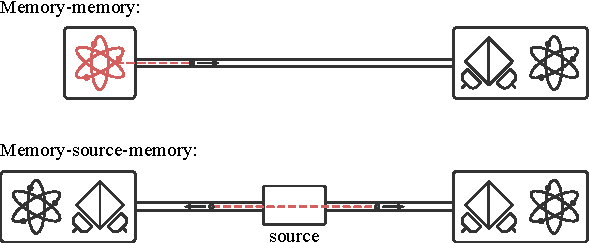
\includegraphics[width=0.85\textwidth]{lesson12/12-2_MM_MSM.pdf}
    \caption[MM and MSM architectures]{Memory-memory and Memory-source-memory link-level architectures.}
    \label{fig:12-2_MM_MSM}
\end{figure}

Figure~\ref{fig:12-2_MM_MSM} shows two more link-leve


\section{Reaching for distance: Entanglement swapping}

% Step Three: Reaching for Distance - Entanglement Swapping

So in the previous step, we have seen how to establish a link-level entanglement. Here we will extend it how to establish long distance end-to-end entanglement. So let's consider that we have three network nodes represented by station zero, station one which is holding two qubits, and station two. And already, we went through the steps of establishing entanglement between the neighbors. So station zero has a qubit which is entangled with a qubit in possession of station one, and also station two has one qubit which is entangled with a different qubit that is in the possession of station one. And the goal is to establish entanglement between station zero and station two.

So how do we do that? Well, what we can do is that we perform a bell state measurement at station one, and depending on the outcome of the measurement what happens is we establish end-to-end long-distance entanglement between station zero and station two, even though they are not directly, physically linked, and this procedure is known as "entanglement swapping", and we will address it- how to derive it mathematically in this step, and in the next step we will address the question of how to handle errors and purify noisy results in order to obtain better quality states between station zero and station two.

So let's label these qubits as follows- station zero has qubit A, station one has qubits  $A'$, which is entangled with A, and qubit $B'$, which is entangled with qubit $B$ at station two, and again end goal is to establish maximal entangled state between station zero and station two, meaning between qubits A and  $B$.

So we said that station zero and station one are entangled via the following Bell pair. And for concreteness let's assume that it's the  \ket{\Phi^+} state, so it's a superposition of \ket{00} plus \ket{11}, and in the same way $B'$ and $B$ are entangled in a maximum entangled state given by  \ket{\Phi^+} which is again \ket{00} plus \ket{11}. So the total state of all the four qubits is given as follows- it's a tensor product of the maximal entangled state  \ket{\Phi^+} between A and  $A'$, and the maximally entangled state  \ket{\Phi^+} between qubits $B'$ and  $B$.

\begin{align}
    \ket{\psi}=\ket{\Phi^{+}}_{A A^{\prime}}\ket{\Phi^{+}}_{B^{\prime} B}
\end{align}

And in the next step, the following identity will be very useful. We can rewrite the state \ket{00} in the Bell state basis, and \ket{00}- you can check for yourself, is just the sum of the maximal entangled state  \ket{\Phi^+} and \ket. Similarly, we can do it for the other states \ket{01}, \ket{10}, and \ket{11}, and they're just different combinations and superpositions of the four Bell states.

\begin{align}
    \begin{aligned}
&|00\rangle=\left(\left|\Phi^{+}\right\rangle+\left|\Phi^{-}\right\rangle\right) / \sqrt{2} \\
&|01\rangle=\left(\left|\Psi^{+}\right\rangle+\left|\Psi^{-}\right\rangle\right) / \sqrt{2} \\
&|10\rangle=\left(\left|\Psi^{+}\right\rangle-\left|\Psi^{-}\right\rangle\right) / \sqrt{2} \\
&|11\rangle=\left(\left|\Phi^{+}\right\rangle-\left|\Phi^{-}\right\rangle\right) / \sqrt{2}
\end{aligned}
\end{align}

So let's get back to our initial state. We said that our initial states are just two Bell states  \ket{\Phi^+} in a tensor product between A -  $A'$ and $B'$ -  $B$. If we write it out, we can we get the following expression in the computational basis, so we have a superposition of four terms. 

\begin{align}
    \begin{aligned}
\ket{\psi}&=\ket{\Phi^{+}}_{A A^{\prime}}\ket{\Phi^{+}}_{B^{\prime} B} \\
&=\frac{1}{2}(|0000\rangle+|0011\rangle+|1100\rangle+|1111\rangle)
\end{aligned}
\end{align}
And now we use our identities. We said that the \ket{00} can be rewritten as a superposition of \ket{\Phi^+} and \ket{\Phi^-}, and here we are going to perform a measurement on $A'$ and $B'$. We are going to measure them in the Bell state basis. This is why we want to rewrite those particular qubits and re-express them from computational basis in the Bell state basis. So, we take \ket{00}, and our identity tells us that we can rewrite it as ( \ket{\Phi^+}, plus \ket{\Phi^-}). Similarly, \ket{01} can be rewritten as the superposition of \ket{\Psi^+} and \ket{\Psi^-}, and so on and so forth. For \ket{10} and the last term \ket{11}. we obtain the following expression,
\begin{align}
    \begin{array}{ll}
=\frac{1}{2 \sqrt{2}}\left(|0\rangle\left(\left|\Phi^{+}\right\rangle+\left|\Phi^{-}\right\rangle\right)|0\rangle\right. \\
+ & |0\rangle\left(\left|\Psi^{+}\right\rangle+\left|\Psi^{-}\right\rangle\right)|1\rangle \\
+ & |1\rangle\left(\left|\Psi^{+}\right\rangle-\left|\Psi^{-}\right\rangle\right)|0\rangle \\
+ & \left.|1\rangle\left(\left|\Phi^{+}\right\rangle-\left|\Phi^{-}\right\rangle\right)|1\rangle\right)
\end{array}
\end{align}

Now we can group the qubits that we are going to measure on the left, and the qubits that we are not going to measure on the right. Here, we're not really doing anything, we're just reordering the qubits in our expression. 

\begin{align}
        \begin{aligned}
|\psi\rangle_{A^{\prime} B^{\prime} A B}=\frac{1}{2 \sqrt{2}} &\left(\left(\left|\Phi^{+}\right\rangle+\left|\Phi^{-}\right\rangle\right)|0\rangle|0\rangle\right.\\
&+\left(\left|\Psi^{+}\right\rangle+\left|\Psi^{-}\right\rangle\right)|0\rangle|1\rangle \\
&+\left(\left|\Psi^{+}\right\rangle-\left|\Psi^{-}\right\rangle\right)|1\rangle|0\rangle \\
&\left.+\left(\left|\Phi^{+}\right\rangle-\left|\Phi^{-}\right\rangle\right)|1\rangle|1\rangle\right)
\end{aligned}
\end{align}

And finally, we group the terms according to which Bell state they are in,
\begin{align}
\begin{aligned}
&|\psi\rangle_{A^{\prime} B^{\prime} A B}=\frac{1}{2 \sqrt{2}}\left(\left|\Phi^{+}\right\rangle(|0\rangle|0\rangle+|1\rangle|1\rangle)\right.\\
&+\left|\Psi^{+}\right\rangle(|0\rangle|1\rangle+|1\rangle|0\rangle)\\
&+\left|\Psi^{-}\right\rangle(|0\rangle|1\rangle-|1\rangle|0\rangle)\\
&\left.+\left|\Phi^{-}\right\rangle(|0\rangle|0\rangle-|1\rangle|1\rangle)\right)
\end{aligned}
\end{align}

So we have the following state-  \ket{\Phi^+} times the superposition, plus \ket{\Psi^+} times the superposition, and so on. So we can now clearly see that if we measure our qubits at station one, which are  $A'$ and $B'$ in the Bell state basis, and we obtain the result corresponding to  \ket{\Phi^+}, then we are projecting the qubits A and B, so the qubits which are held in station zero and station two, into a maximally entangled Bell state,  \ket{\Phi^+} (\ket{00} plus \ket{11}). Similarly we have a possibility of obtaining the other three possible Bell states, at  $A'$ and $B'$ we can get \ket{\Psi^+}. Then we know that the state of qubits A and $B$ is also in \ket{\Psi^+}, and similarly for \ket{\Psi^-} and \ket{\Phi^-}.

So again, let's go back to our visual aid. We started with two maximally entangled pairs of qubits between station zero and station one, and between station two and station one. Then we performed a Bell state measurement on the qubits held by station one, and this resulted in the entanglement being established between the end-to-end nodes, station zero and station two.

But that's not all. Station one also needs to let station zero and station two know of the outcomes of the measurements. It doesn't need to send the outcome of the measurements to both of the stations. It is enough to send it just to one, but both of the stations need to be notified that the procedure has been carried out successfully. So this introduces some time delay between how far we can progress in terms of establishing entanglement, because this station zero and station two need to know that now they are entangled. They need to be notified classically that the Bell state measurement at station two has taken place and it has been carried out successfully.

Maybe you have noticed that the procedure that we have been describing in this step is very similar to the procedure described in step two, where we are establishing link-layer entanglement, and in fact, mathematically it's very similar. In link-level entanglement, we're dealing of swapping the entanglement between photon and memory, by measuring the photons at the Bell state analyzer and establishing a memory-to-memory entanglement, whereas in end-to-end entanglement we are only entanglement swapping between entanglement established between pairs of memories. And this is physically quite a big difference because using linear optics, we will see in the next lesson, the maximum success probability of actually performing entanglement swapping on photons is limited by fifty percent, whereas entanglement swapping between memories can be done deterministically, provided that we have good experimental techniques and we can limit the effects of noise.

An alternative way of understanding entanglement swapping is via teleportation. Remember, in teleportation, we are in possession of some arbitrary state. So let's say that our state is this qubit $A'$, and then what we do is we share a maximally entangled state between qubits $B'$ and B, and by measuring these two qubits $A'$ and $B'$ in the Bell state basis, we are effectively sending the qubit  $A'$ on to the qubit that was originally labeled as  $B$. So we are transferring the state that  $A'$ was in onto B, and then $B$ becomes $A'$. But $A'$ was entangled with A, so basically it takes its entanglement and it carries it all the way to $B$. This is another very neat way of understanding entanglement swapping.

\section{Detecting errors: purification}
\label{sec:purification}

% Step Four: Detecting Errors - Purification

In this step, we will address what happens when we also include errors into our considerations, and how we can handle them and create a state between station zero and station two that's of acceptable quality. So our desired state that we want to share between states station zero and two is given by the maximally entangled state $\ket{\Phi^+}$. In the density matrix form, we can just write it as the outer product in this form. 
\begin{align}
    \rho=\left|\Phi^{+}\right\rangle\left\langle\Phi^{+}\right|
\end{align}
But in reality, there will always be some noise that are spoiling our operations. So we will not end up with the pure state  \ket{\Phi^+}. In fact, what we will have is, with some probability given by the fidelity $F$, we will have the state  \ket{\Phi^+}, and that will be mixed with some noise terms, with probability given by $1-F$, 
\begin{align}
    \rho=F\left|\Phi^{+}\right\rangle\left\langle\Phi^{+}|+(1-F)| \text {noise}\right\rangle\langle\text {noise}|.
\end{align}

So the question now is, "How can we detect it and how can we correct it?"

Here, we will represent the noisy Bell state by slightly misaligned arrows, like that.

Rather than considering the full general case of how noise affects our maximally entangled state, we will consider just one example and that's the flip channel. Now this channel we have seen in Lesson three Step three, and it goes as follows- we have our input pure state psi, and let's say that it travels through a noisy channel represented by this noisy fiber, and at the end of the output we can get two outcomes and only two outcomes. One is the intended pure state psi and we get it with probability (one minus p), and the other one is a different state where we apply the flip operation represented by the Pauli X matrix, so with probability p we get a state that's flipped, so X times state psi. And mathematically we represent this output as a density matrix in the following form,
\begin{align}
    \rho=(1-p)|\psi\rangle\langle\psi|+p X| \psi\rangle\langle\psi| X.
\end{align}
So with probability one minus p, we have our intended desired state psi, and with probability p we have the state psi but flipped where we applied the matrix Pauli X. So for example, if our input state is a zero, $|\psi\rangle=|0\rangle$,
then the output state will have the following form,
\begin{align}
    \rho=(1-p)|0\rangle\langle 0|+p| 1\rangle\langle 1|=\left(\begin{array}{cc}
1-p & 0 \\
0 & p
\end{array}\right).
\end{align}
If we just substitute zero for psi, we get the following expression, which in matrix form can be written as this. It only has two diagonal terms, with probability $1-p$ it's in zero, and with probability $p$ it's in a one. On the other hand, if our input state is one, $|\psi\rangle=|1\rangle$, then our output state is given by this expression
\begin{align}
    \rho=(1-p)|1\rangle\langle 1|+p| 0\rangle\langle 0|=\left(\begin{array}{cc}
p & 0 \\
0 & 1-p
\end{array}\right)
\end{align}
where with probability one minus p, we get one, and with probability p we flip it back to zero. So again, it's a diagonal matrix but this time the probabilities are flipped.

So, how is our Bell state affected by this flip channel? Well, we said that at the end our output state is given by this form
\begin{align}
    \rho=F\left|\Phi^{+}\right\rangle\left\langle\Phi^{+}|+(1-F)| \text {noise}\right\rangle\langle\text{noise}|.
\end{align}
With some probability given by the fidelity $F$, we've got our desired maximally mixed state  \ket{\Phi^+}, and with some probability $1-F$, we've got some noise terms. But now, we are considering the particular example of a bit flip channel, so our noise term is only given by X applied to the state  \ket{\Phi^+}. Now- but remember, the state  \ket{\Phi^+} actually has two qubits, so where are we applying the flip? Where are we applying the Pauli X operator? Actually it doesn't matter where we apply it, as long as it's just one qubit, so we may apply it on qubit one or we may apply it on qubit two. In both cases, we will still end up with the following state,
\begin{align}
\begin{aligned}
\rho &=F\left|\Phi^{+}\right\rangle\left\langle\Phi^{+}|+(1-F) X| \Phi^{+}\right\rangle\left\langle\Phi^{+}\right| X \\
&=F\left|\Phi^{+}\right\rangle\left\langle\Phi^{+}|+(1-F)| \Psi^{+}\right\rangle\left\langle\Psi^{+}\right|
\end{aligned}
\end{align}
with some probability given by the fidelity $F$, we've got our intended state  \ket{\Phi^+}, and with probability $1-F$ we've got some noisy term represented by state \ket{\Psi^+}, because if we apply X to one of the qubits of  \ket{\Phi^+}, we obtain state \ket{\Psi^+}. Now keep in mind that this is just one possible source of error out of many, many possibilities. You could have many other unitary errors, or you could also have non-unitary errors, but here we just want to keep it simple. If you are interested in all of the sources of other errors, we recommend you look at some literature on quantum error correction. So we said that we would like to detect the errors and correct the errors. One way of doing that is using "quantum error correction", but usually this comes with a large overhead in terms of qubits, and also in terms of operations. In here, we will look at a more simple and less ambitious ambitious procedure known as "purification". And in this process, we will see that we can easily detect whether error has occurred or not, and after the procedure we will end up with some probability in the intended state  \ket{\Phi^+}, even if some errors have occurred during the process. The point is that we would like to know the information, like- has our ideal state been affected by noise or not? One way is to measure the state, but of course this destroys the entanglement in the state. So we have to be very careful how we handle and how we obtain the information about what our state is in. So we need to do this procedure of purification without destroying our state. If we destroy it, then we cannot establish entanglement between end-to-end nodes.

And another complication is that these qubits are not held locally by one player, let's say Alice or Bob. They're held in two different network nodes, so they are far apart, maybe tens of kilometers apart, so we have to keep that in mind.

So, the solution is to use another Bell pair, and use this other Bell pair to learn some information about the Bell pair that we are trying to purify. So we have the following scenario- we still have station zero and station two, but this time we have two copies of a noisy Bell pair that the stations share between each other. Previously, we have seen how we can establish this end-to-end entanglement. So let's say that we've done it twice, and we know that we are sharing two copies of a noisy Bell state, then Alice and Bob, they can apply some local operations on their qubits, and soon we will see what those operations are. By doing these two qubit operations, and then performing some measurements, they can actually find out information about one of their entangled pairs without destroying the entanglement between them and correct it so that the end result- the end state that's shared between station zero and two is of higher quality in terms of the fidelity. So let's see how that works.

Here these wires, these two horizontal wires, represent Bell pairs shared between Alice and Bob. So we've got state  \ket{\Phi^+} one and state  \ket{\Phi^+} two, or at least these are the ideal state that we would like to share. Of course, in real life they will be noisy. And then time flows on. For Alice, it flows from right to left, meaning first she applies a CNOT gate on her qubits, where the first qubit that she has is the control and the second qubit is the target. On Bob's side, the time flows from left to right, so again, meaning first he applies a CNOT on his qubits where the first one is control and the second one is target again, then both of them, Alice and Bob, they measure their second qubit in the Z basis. They obtain their measurements, which is either zero or one, and then they exchange this classical information with each other.

And this is how we can represent it mathematically. So we start with a state \ket{\Psi^+}, and \ket{\Psi^+} so in tensor product. This \ket{\Psi^+} shared is the first pair shared between Alice and Bob, and this is the second pair shared between Alice and Bob. We can expand it out, and for clarity we are omitting the normalization factor. So, we obtain the initial state in the following form- we've got a superposition of four terms. Then we apply the control-NOT gate on Alice's qubits, so we are applying the control-NOT gate between the first qubit and the third qubit,
\begin{align}
    \begin{aligned}
\left|\Phi^{+}\right\rangle_{1}\left|\Phi^{+}\right\rangle_{2} &=(|00\rangle+|11\rangle)(|00\rangle+|11\rangle) \\
=&|00\rangle|00\rangle+|00\rangle|11\rangle+|11\rangle|00\rangle+|11\rangle|11\rangle \\
\stackrel{\mathrm{CNOT}_{A}}{\longrightarrow} &|00\rangle|00\rangle+|00\rangle|11\rangle+|11\rangle|10\rangle+|11\rangle|01\rangle \\
\stackrel{\mathrm{CNOT}_{B}}{\longrightarrow} &|00\rangle|00\rangle+|00\rangle|11\rangle+|11\rangle|00\rangle+|11\rangle|11\rangle \\
&=\left|\Phi^{+}\right\rangle_{1}\left|\Phi^{+}\right\rangle_{2}
\end{aligned}.
\end{align}
They represent the qubits that are on Alice's side. So here for this term, we've got Alice's qubits in the state \ket{00}, so the CNOT doesn't change them. For the second term, they are \ket{01}, so again nothing changes. Whereas for the next case, Alice's qubit is in one and zero, therefore the CNOT gate transforms it into \ket{11}, and similarly for the last term, and then we apply the CNOT on both sides and we obtain the following expression. We see that nothing has really changed, and in fact we again obtain two Bell pairs shared between Alice and Bob, and now after the measurement of the second Bell pair we know that since they are in the state  \ket{\Phi^+}, the measurements have to be correlated, so with equal probability they can obtain \ket{00} or \ket{11}, but they cannot obtain anti-correlated results.

So, by exchanging the classical information between Alice and Bob, they can check if their results are correlated or not. If they are correlated, they keep the first pair of qubits. If they are not correlated, they just discard them. So let's say that no error has occurred on our Bell pairs, so our pair one is in the ideal state  \ket{\Phi^+}, and our pair two is also in the ideal state  \ket{\Phi^+}. This happens with probability f squared. When they go through the purification procedure, the measurement results can only be \ket{00} or \ket{11}. They are correlated, therefore they agree, therefore Alice and Bob keep their first Bell pair. Remember, the second belt pair is destroyed by the measurement. And at the end, they end up with a state  \ket{\Phi^+}. This is not so surprising because they already started with the ideal case  \ket{\Phi^+}, so, therefore purification should work, but let's consider the case where a bit flip error has occurred on both pairs. So we're considering this last row in the column. Alice and Bob are sharing two pairs of the state \PsiPlus, so it's not their ideal intended state. This can occur with probability one minus f squared, but again if we go through the whole procedure of applying the CNOT gates and then measuring the second pair of qubits in the Z basis, we can again check that we obtain correlated results \ket{00} and \ket{11}. These again- they agree, therefore we keep the first pair of qubits. So the success probability of this procedure is given by the expression $F^2+(1-F)^2$.

\begin{tabular}{|l|l|l|l|l|l|l|}
\hline Pair 1 & Pair 2 & Prob. & Meas. result & Agree? & Action & Result \\
\hline$\left|\Phi^{+}\right\rangle$ & $\left|\Phi^{+}\right\rangle$ & $F^{2}$ & 00 or 11 & Y & Keep & $\left|\Phi^{+}\right\rangle$ \\
\hline$\left|\Phi^{+}\right\rangle$ & $\left|\Psi^{+}\right\rangle$ & $F(1-F)$ & 01 or 10 & N & Discard & N/A \\
\hline$\left|\Psi^{+}\right\rangle$ & $\left|\Phi^{+}\right\rangle$ & $(1-F) F$ & 01 or 10 & N & Discard & N/A \\
\hline$\left|\Psi^{+}\right\rangle$ & $\left|\Psi^{+}\right\rangle$ & $(1-F)^{2}$ & 00 or 11 & Y & Keep & $\left|\Psi^{+}\right\rangle$ \\
\hline
\end{tabular}

Therefore, the output fidelity given by $F'$ equals the ratio of $F^2$ to the success probability,
\begin{align}
    F^{\prime}=\frac{F^{2}}{F^{2}+(1-F)^{2}}.
\end{align}
Now you can notice that if the initial fidelity $F$ is larger than 0.5, then the new obtained fidelity actually increases: $F' > F$ when $F > 0.5$. This is why this procedure is called purification. We start with some initial amount of the fidelity, and we want to get it as high as possible, so what we do is we take two noisy states and we apply the purification, and with some success probability we obtain only one state but of higher fidelity. Of course you can have more and more pairs of states and keep applying purification, and this way you increase the fidelity of the end pairs even further.

This is just a simple example of purification, and does not cover all of the operational details. You can learn more from advanced materials, such as research papers, Professor Van Meter's first book, or future modules that we will be creating.

\section{Making a network}

% Step Five: Making a Network

So far, we have considered how to create entanglement between neighboring nodes, so link-level entanglement, how to extend this with entanglement swapping to end-to-end entanglement, so entanglement between nodes that are not physically connected directly. Now let's consider what it takes to actually create a network. There are a few problems, but the two main problems that we will consider in this step are routing (how you direct traffic through a network), and also multiplexing and resource management.

Let's say that we've got some complicated network like this, and we wish to communicate from this point over here, all the way down to this point over there. The job of a network is to establish a connection between those two nodes. In quantum networks, we wish to establish an entangled pair between those two nodes such that we can either use it for some quantum key distribution, or for teleportation, or for any other purposes we may wish to consider. So how does the network know how to do it? Well, it has to first content with the first problem, that's routing.

How does it pick a particular path where it performs entanglement swapping? Well, let's consider a simpler case of the following network- so let's say that we want to communicate from A to E. We can see that there are three different possible paths that the network can take. It can establish an entangled pair between A and E by performing entanglement swapping at B, or it can do it by entanglement swapping between D while it's sharing link-level entanglement between D-E and A-E, or it can go via the node C and perform entanglement swapping there, as well as D. So first it needs to establish link-level entanglement between A-D, D-C, C-E, and then perform entanglement swapping on the qubits at C and entanglement swapping on the qubits at D in order to establish end-to-end entanglement between A and E.

What we need in order to evaluate which way is best, is to look at the cost that it takes to establish link-level entanglement, and then how to combine these costs in order to establish the cost for the entire path, so for the entire end-to-end entanglement. So one possible way of evaluating the link-level entanglement is to evaluate the cost of establishing a link-level entanglement- is seconds per bell pairs at a threshold fidelity. So what does that mean? As we said, in order to establish entanglement, let's say between A and B, we have to first make the quantum memories that are sitting at A emit a photon, and quantum memory sitting at $B$ to emit a photon, and then they have to meet, let's say in the middle, if we are considering the memory interference- memory setup where the photons can be measured in a Bell state basis, and that will entangle the memories at A and at B, but these photons will get lost in the fiber- they will get attenuated. So this procedure is not deterministic. Sometimes we get lucky and the link-level entanglement can be established quickly. Sometimes we have to wait a little bit longer. So the more lossy the channel is, the more lossy the fiber is, the more we are expected to wait a little bit longer for the Bell pairs to get established. And in order to make this comparison fair, we set a fixed fidelity, that we are looking to establish bell pairs at a given fidelity, and this is usually dictated by the protocol that we want to run, or for by the end-to-end distance between the nodes A and E. So this gives us a good idea for a cost of establishing the link-level entanglement. Now, how do we combine these costs for each individual links in order to know the full cost of establishing end-to-end entanglement over a longer path? Well, one possibility is to use Dijkstra's shortest path first algorithm. So what we can do is we can sum the costs for the path A-B-E in order to obtain a good estimate of the full total cost of establishing end-to-end entanglement, or we can do it for A-D-E and A-D-C-E. This way the network can know what's actually best, and it will be able to deliver the entire end-to-end entanglement more efficiently. And by knowing which path is most efficient, of course it knows how to route information and establish an end-to-end entanglement.

So the next problem that we have to deal with is multiplexing, and that can be demonstrated by considering the following scenario- we've got a bunch of nodes over here that are all connected to a node E, and here on the right side again, we've got the following tree that's leading to node F. So let's say that A is trying to communicate with K. Well, we can use link-level entanglement between E-F, F-K, and A-E, and then apply entanglement swapping at E, entanglement swapping at F, in order to obtain end-to-end entanglement between A-K. But what if different two nodes also are trying to communicate? Let's say that $B$ wants to establish end-to-end entanglement with node J. They have to go through the link E-F. This creates contention on E-F link, so the network needs to know how to handle such requests where a single link has to be shared between two different pairs- between pair A-K and B-J.

Furthermore, we can have more network nodes trying to establish end-to-end entanglement. This case, we can have C-H, C and H, or we can even have the case where we have node G trying to communicate with node K, and this creates contention on the following link, on the link F-I, that the network needs to know how to handle such requests.

In this lesson, we have seen the four requirements for building a quantum network. So first we started at the bottom with a basic building block, and that's how to establish entanglement between two neighboring nodes of a network, meaning establishing link-level entanglement and how to handle photon losses. Next, we saw how we can establish end-to-end entanglement, meaning entanglement between nodes which don't share a direct physical link using entanglement swapping. Then we talked about how to handle errors, how to improve the quality of our distributed state, and namely we introduced the protocol of purification, and finally in this last step we gave you a little bit more idea what it takes to build the network that there are other considerations that we have to take into account, such as routing, multiplexing and resource management. But this is all just building a single network. Quantum Internet is a different beast entirely. Quantum Internet is a network of quantum networks, so that we will discuss in the coming lessons.


\newpage
\begin{exercises}
\exer{Consider the following quantum state:}
\begin{equation*}
\ket{\psi} = \frac{\sqrt{3}}{2}\ket{0} + \frac{1}{2}\ket{1}
\end{equation*}
\subexer{Find the probability of measuring a zero.}
\subexer{Find the probability of measuring a one.}


\end{exercises}

